\documentclass[numbers=noenddot]{thesis}
\usepackage{tikz}

% hier namen etc. einsetzen
\fullname{Lukas Stöferle, Ferdinand Birk, Marius Kircher}
\email{lukas.stoeferle@uni-ulm.de, ferdinand.birk@uni-ulm.de, marius.kircher@uni-ulm.de}
\headline{Mobile Application Lab - FancyQuartett\\Dokumentation}
\titel{}
\jahr{WS 2015/16}
\matnr{}
\gutachterA{Prof. Dr. Manfred Reichert}
\gutachterB{Marc Schickler}
\betreuer{Marc Schickler}
\typ{Dokumentation}
\fakultaet{Ingenieurwissenschaften, Informatik und \\Psychologie}
\institut{Institut für Datenbanken und Informationssysteme}

% Falls keine Lizenz gewünscht wird bitte den folgenden Text entfernen.
% Die Lizenz erlaubt es zu nichtkommerziellen Zwecken die Arbeit zu
% vervielfältigen und Kopien zu machen. Dabei muss aber immer der Autor
% angegeben werden. Eine kommerzielle Verwertung ist für den Autor
% weiter möglich.
\license{

}

\hypersetup{%
	pdftitle=\pdfescapestring{\thetitel},
	pdfauthor={\thefullname},
 	pdfsubject={\thetyp},
}


% trennungsregeln
\hyphenation{Sil-ben-trenn-ung}

\usetikzlibrary{trees}
\begin{document}
\frontmatter
\maketitle
% impressum
\clearpage
\impressum

\cleardoublepage
% ab hier zeilenabstand 1,4 fach 10pt/14pt
\setstretch{1.4}

% tabellen zeilenabstand
\renewcommand{\arraystretch}{1.5}


% inhaltsverzeichnis einfügen
\tableofcontents

\mainmatter
% hier kommen die kapitel der arbeit
\chapter{Einleitung}
\label{cha:einleitung}

Seit der Ankündigung des weltweit ersten Smartphones durch \textit{Apple Inc.} im Jahre 2007 hat sich sehr viel auf dem Markt für mobile Endgeräte getan. Heute gibt es eine Vielzahl an verschiedenen Smartphones von unterschiedlichen Herstellern, die jeweils mit unterschiedlichen Betriebssystemen ausgestattet sind, wie z.B. \textit{Android} von \textit{Google Inc.}, \textit{iOS} von \textit{Apple Inc.} oder \textit{WindowsPhone} von \textit{Microsoft}. Smartphones sind heute nicht mehr aus unserem Alltag wegzudenken, da sie den Benutzer aufgrund ihrer Mobilität und dank verschiedener Applikationen (kurz \glqq Apps\grqq) unterstützen aber auch unterhalten. Im diesjährigen Anwendungsfachs \textit{Mobile Application Lab} entstand deshalb im Rahmen eines kleinen Softwareprojektes eine Quartett-App, die sich durch eine beliebige Anzahl an auswählbaren Kartendecks von den bereits existierenden Apps im App-Store abheben soll. Hierbei werden Kartendecks per \textit{Representational State Transfer (REST)} von einem Server der Universität Ulm heruntergeladen, die dann auf dem Gerät persistent gespeichert werden und somit auch offline verfügbar sind. Neben den vorgegebenen Anforderungen durfte jedes Team eigene Ideen einbringen, was zu unterschiedlichen Anwendungen führte.

\section{Motivation}
\label{sec:motivation}

Apps spielen heute, aber auch in Zukunft eine große Rolle im mobilen Software-Bereich. Durch die Programmierung einer Quartett-App in Teams soll mehr Praxiserfahrung in das doch eher theorielastige Studium mit einfließen. Die Quartett-App deckt möglichst viele Bereiche der App-Programmierung ab, wodurch die Teams später in der Lage sind, ihre eigenen Ideen und Anwendungen planen und umsetzen zu können.

\section{Kontext}
\label{sec:kontext}

Die Quartett-App wird im Auftrag des \textit{Institut für Datenbanken und Informationssysteme} der \textit{Universität Ulm} entwickelt. Dabei sollen die Teams grundlegende Werkzeuge zur App-Programmierung kennenlernen und somit Schritt für Schritt die benötigten Schritte der App-Entwicklung meistern. Durch sorgfältige Planung, wie z.B. mit Hilfe von Mockups oder Diagrammen, soll die spätere Implementierung vereinfacht werden. Neben der Planung und Implementierung der Anwendung sollen die Teams sich mit den Besonderheiten der Zielplattform und der dazugehörigen Smartphones (wie z.B. Datenhaltung, Sensorik oder gestenbasierter Eingabe) auseinander setzen.



\chapter{Anforderungen}
\label{cha:anforderungen}

% TODO

\section{funktionale Anforderungen}
\label{sec:funtionaleanforderungen}

% TODO

\section{nicht-funktionale Anforderungen}
\label{sec:nichtfunktionaleanforderungen}

% TODO
\chapter{Architektur}
\label{cha:architektur}

% TODO
\chapter{Implementierung}
\label{cha:implementierung}


% TODO ... kleine Einleitung (siehe vorherige Kapitel)
Die Anwendung wurde in \emph{Android Studio 1.5.1} implementiert. Zur Versionsverwaltung wurde ein bei Github gehostetes Git-Repository verwendet. Als Unterstützung beim Anbinden der REST-API wurde die Google Chrome-Erweiterung \emph{Advanced Rest Client (ARC)} verwendet, welche es erlaubt RAW-HTTP Requests abzusetzen und anschließend die Antwort in Plaintext anzuzeigen.

\section{Vorgehensweise}
In der Implementierungsphase wurden zuerst die Datenklassen implementiert und mit den Standard Getter und Setter ausgestattet. Darauf aufbauend wurde die Implementierung in Gameentwicklung, Deckmanagemant und Statistikmanagemant eingeteilt und fortan parallel implementiert. 


\section{Datenhaltung}
Für die Speicherung der Deckdaten, welche aus Text- und Bilddaten bestehen, haben wir uns für die Variante des Dateisystems im internen Speicher entschieden. Da wir die Deckdaten als JSON erhalten, bietet es sich an, diese nach spezifizierten Modifikationen auch wieder als JSON zu speichern und erreichen so eine gewisse Konsistenz in den \emph{OfflineDeck- und OnlineDeckLoadern}. Es wäre ein nicht unwesentlicher Mehraufwand gewesen, eine entsprechende Datenbankklasse zu schreiben, die mittels SQL-Statements die JSON-Daten in einem eigenen Schema persistiert speichert. 

Für die Speicherung der Spielzwischenstände und der Statistiken wird Androids Konzept der \emph{Shared Preferences} genutzt. Dies sind Key-Value Paare welche in dem \emph{shared\_prefs} Ordner einer jeden App als XML gespeichert werden. Sollen Objekte abgespeichert werden wie z.B. die Spielzwischenstände, dann müssen diese Objekte serialisiert sein. Da wir zum Speichern des aktuellen Spielzustandes ganz einfach das \emph{GameEngine}-Objekt abspeichern impliziert dies, dass unsere \emph{GameEngine}-Klasse das Interface \emph{Serializable} implementiert. Das betrifft nicht die Controller der GameEngine, weshalb diese bei jedem "Resume" neu initialisiert werden müssen, da sie nicht mit serialisiert werden.

\begin{figure}[!ht]
\centering
\tikzstyle{every node}=[draw=black,thick,anchor=west]
\tikzstyle{selected}=[draw=red,fill=red!30]
\tikzstyle{optional}=[dashed,fill=gray!50]
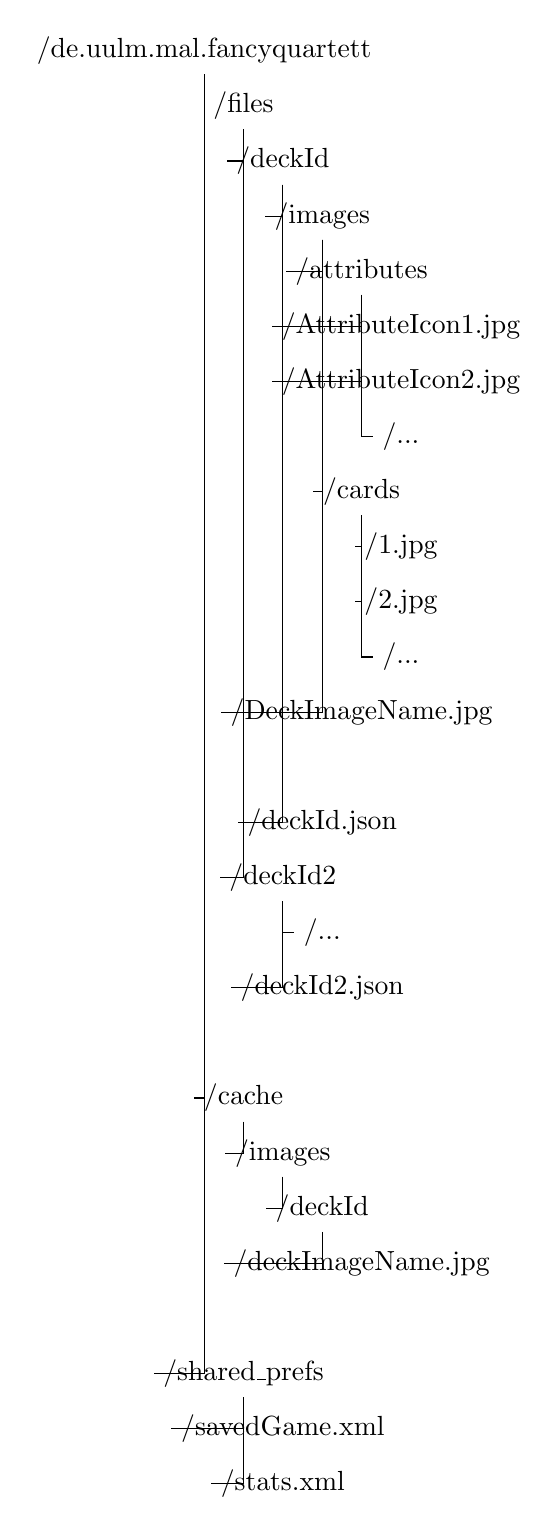
\begin{tikzpicture}[%
  grow via three points={one child at (0.5,-0.7) and
  two children at (0.5,-0.7) and (0.5,-1.4)},
  edge from parent path={(\tikzparentnode.south) |- (\tikzchildnode.west)}]
  \node {/de.uulm.mal.fancyquartett}
    child { node  {/files}
      child { node  {/deckId}
        child { node {/images}
          child { node {/attributes}
            child { node {/AttributeIcon1.jpg}}
            child { node {/AttributeIcon2.jpg}}
            child { node {/...}}
          }
          child [missing] {}				
          child [missing] {}				
          child [missing] {}
          child { node {/cards}
            child { node {/1.jpg}}
            child { node {/2.jpg}}
            child { node {/...}}
          }
          child [missing] {}				
          child [missing] {}				
          child [missing] {}
          child { node {/DeckImageName.jpg}}
        }
        child [missing] {}				
        child [missing] {}				
        child [missing] {}
        child [missing] {}				
        child [missing] {}				
        child [missing] {}
        child [missing] {}				
        child [missing] {}				
        child [missing] {}
        child [missing] {}
        child { node {/deckId.json}}
      }
      child [missing] {}				
      child [missing] {}				
      child [missing] {}
      child [missing] {}				
      child [missing] {}				
      child [missing] {}
      child [missing] {}				
      child [missing] {}				
      child [missing] {}
      child [missing] {}				
      child [missing] {}				
      child [missing] {}				
      child { node {/deckId2}
        child { node {/...}}
        child { node {/deckId2.json}}
      }
    }
      child [missing] {}				
      child [missing] {}				
      child [missing] {}
      child [missing] {}				
      child [missing] {}				
      child [missing] {}
      child [missing] {}				
      child [missing] {}				
      child [missing] {}
      child [missing] {}				
      child [missing] {}				
      child [missing] {}
      child [missing] {}				
      child [missing] {}
      child [missing] {}				
      child [missing] {}
      child [missing] {}				
    child { node {/cache}
      child { node {/images} 
      	child { node {/deckId}
	  child { node {/deckImageName.jpg}}
    	}
      }
    }
      child [missing] {}				
      child [missing] {}
      child [missing] {}				
      child [missing] {}	
    child { node {/shared\_prefs}
      child { node {/savedGame.xml}} 
      child { node {/stats.xml}}
    };

\end{tikzpicture}

    \caption{Ordnerstruktur im Dateisystem}
    \label{fig:folderstructure}

\end{figure}

Ein heruntergeladenes Deck wird wie in Abbildung \ref{fig:folderstructure} auf dem Dateisystem abgelegt. Durch diese exakt spezifizierte Struktur ist es möglich einfache \emph{LocalDecksLoader} bzw. \emph{LocalDeckLoader} zu implementieren. Da die Daten intern unter 
\begin{align*}
\emph{/data/data/[packagename]/files/}
\end{align*}
gespeichert werden kann eine manuelle Veränderung der Daten ohne gesonderte Root-Rechte ausgeschlossen werden und daher für den Zweck dieses Spiels als geeignet angesehen werden.

Die Klasse \emph{Image} aus Abbildung \ref{fig:datenmodell} ist nicht wirklich ein Bild sondern lediglich eine Wrapper-Klasse für die Informationen des zugehörigen Bildes. Hier wird zur Laufzeit festgehalten, ob und wo das Bild lokal ist, sowie die Onlineadresse wo es im Zweifel nachgeladen werden kann. Die Klasse enthält eine Methode \emph{getBitmap()} welche dann aus dem lokalen Pfad mit der Klasse \emph{BitmapFactory} ein \emph{Bitmap}-Objekt decodiert und zurückgibt.


\section{Datenverarbeitung}
In der Implementierung der Datenklassen für die Decks wird wie in Abbildung \ref{fig:datenmodell} zu sehen zwischen \emph{OfflineDeck} und \emph{OnlineDeck} unterschieden. So ist es nicht nötig in der Deckliste für alle verfügbaren Decks alle vorhandenen Daten herunterzuladen. Alle Dateioperationen werden in gesonderte Loader ausgelagert, welche alle von der Klasse \emph{AsyncTask} erben und somit parallel zum UI-Thread laufen.

Der \emph{OnlineDecksLoader} fragt lediglich die \emph{/decks} Ressource ab um an die IDs der vorhandenen Decks zu kommen über welche dann in einem zweiten Request nach \emph{decks/ID} der Name, Beschreibung und der Pfad für das Coverbild abgefragt werden. Das Coverbild wird anschließend vom gegebenen Pfad heruntergeladen und mittels der Methode \emph{decodeStream()} der Klasse \emph{BitmapFactory} in ein \emph {Bitmap}-Objekt umgewandelt. Dieses wird dann in den Cachepfad (siehe Abbildung \ref{fig:folderstructure}) abgelegt und fortan nichtmehr extra angefragt. Er gibt anschließend eine Liste von fertigen OnlineDecks an seine Listener zurück.

Der \emph{DeckDownloader} kapselt hingegen die ganze Logik des Downloads bis hin zur persistenten Speicherung der gesamten Deckdaten eines über die ID spezifizierten Decks. Er ruft dazu sequentiell hintereinander die verschiedenen Ressourcen-Pfade aus Abschnitt \ref{sec:netzwerkfunktionen} ab, ändert nach erfolgreichem Download der Bilder den Bildpfad in den JSON-Objekten und berechnet zusätzlich über allen Attributwerten der Karten jeweils den Median und hängt diesen direkt in die einzelnen Attribute. Anschließend werden alle JSON-Teile zu einem großen JSON-Objekt kombiniert und als File im Dateisystem gespeichert. Zusätzlich wird direkt ein OfflineDeck erstellt und an die Listener zurückgegeben.

\section{Spiellogik}

Wie bereits im Abschnitt \ref{sec:activities_in_fancyquartett} erläutert wird in der \emph{GameActivity} das Spiel ausgeführt. Sie beinhaltet ein Objekt der Klasse \emph{GameEngine}, welche mit Hilfe der an die \emph{GameActivity} übergebenen Parameter initialisiert wird. Die wichtigen Komponenten der \emph{GameEngine} sind in der Abbildung \ref{fig:architecture_gameengine} dargestellt.

\begin{figure}[ht]
\centering
    \includegraphics[trim=0 280 220 0,width=\textwidth]{../img/ArchitekturGameengine.pdf}
    \caption{Aufbau der GameEngine Klasse}
    \label{fig:architecture_gameengine}
\end{figure}

Im Folgenden werden die Komponenten aus Abbildung \ref{fig:architecture_gameengine} kurz erläutert:

\begin{itemize}
\item{\textbf{Player}\quad 
Jeder Spieler wird in einem Player-Objekt gespeichert.
}
\item{\textbf{OfflineDeck}\quad
Das Kartendeck welches im aktuellen Spiel verwendet wird.
}
\item{\textbf{Tasks}\quad
Hierbei werden verschiedene Typen verwendet, welche von der Klasse \emph{AsyncTask} erben:
	\begin{itemize}
	\item{\textbf{SoftKiTask}\quad
	Einfacher Computergegner, der einen Spielzug ausführt.
	}
	\item{\textbf{MediumKiTask}\quad
	Mittlerer Computergegner, der einen Spielzug ausführt.	
	}
	\item{\textbf{HardKiTask}\quad
	Schwerer Computergegner, der einen Spielzug ausführt.
	}
	\item{\textbf{PlayerTimeoutTask}\quad
	Zählt die Zeit herunter, die ein Spieler pro Zug zur Verfügung hat. Falls die Zeit abgelaufen ist wird ein beliebiges Attribut gewählt.
	}
	\item{\textbf{GameTimeTask}\quad
	Zählt die Zeit herunter, die für ein Spiel festgelegt wurde.
	}
	\end{itemize}
\item{\textbf{Controller}\quad
Hierbei wurden verschieden Typen verwendet:
	\begin{itemize}
	\item{\textbf{CardController}\quad
	Regelt die Kartenverteilung zu jedem Zeitpunkt des Spiels. 
	}
	\item{\textbf{PlayerController}\quad
	Regelt die Punkteverteilung und ist für die Festlegung des Gewinners zuständig.
	}
	\item{\textbf{StatisticController}\quad
	Regelt die Statistiken und schreibt diese in die \emph{Shared Preferences}
	}
	\end{itemize}
}
\item{\textbf{FragmentManager}\quad
Ist dafür zuständig dass nach jeder Runde eine neue Karte angezeigt wird.
}
}
\end{itemize}

Das komplette Spiel beruht auf dem \emph{Listenerkonzept}, d.h. es gibt keine Schleife die dauerhaft nach Ereignissen sucht. Somit ist wird z.B. nach jedem Spielzug oder nachdem ein Dialogfenster geschlossen wurde eine Nachricht an die \emph{GameEnginge} gesendet, die dann weitere Funktionen aufruft.


\section{Views}
Die Views der in Abschnitt \ref{sec:activities_in_fancyquartett} erläuterten Activities sind allesamt als Fragment implementiert. Jede Activity enthält also mindestens ein Fragment, in welchem das eigentliche Layout ausgerollt wird. Rückwirkend war das für dieses Projekt wohl ein unnötiger Zusatzaufwand, da das Game aktuell nur für Smartphones optimiert ist. Der Vorteil alles mit dem Fragment-Konzept zu implementieren hätte sich unter anderem erst ausgewirkt, wenn das Game auch für andere Formfaktoren wie z.B. Tablets hätte optimiert werden müssen, denn dann hätte das Layout mithilfe der Fragments sehr leicht angepasst werden können. Obwohl dies keine direkte Anforderung war wollten wir uns diese Option trotzdem offen halten.





\chapter{Anforderungsabgleich}
\label{cha:anforderungsabgleich}

In der folgenden Tabelle soll verdeutlicht werden, wie gut die an die App gestellten Anforderungen umgesetzt wurden. Die verwendete Skala geht von \glqq sehr gut\grqq\ (1) bis \glqq ungenügend\grqq\ (6). Außerdem wird im Folgenden noch einmal auf jede Anforderung konkret eingegangen.

\section{Funktionale Anforderungen}
\label{sec:abgleich_funtionaleanforderungen}

\begin{table}[ht]
\centering
\begin{tabular}{l|c c c c c c}
funktionale Anforderungen & 1 & 2 & 3 & 4 & 5 & 6 \\ \hline\hline
Spieltyp & $\checkmark$ &  &  &  &  &   \\
Spielmodi & $\checkmark$ &  &  &  &  & \\
Schwierigkeitsgrade & $\checkmark$ &  &  &  &  & \\
Einstellungsmöglichkeiten & $\checkmark$ &  &  &  &  & \\
Gespeichertes Spiel & $\checkmark$ &  &  &  &  & \\
Statistiken & $\checkmark$ &  &  &  &  & \\
Galerie & $\checkmark$ &  &  &  &  & \\
Kartendecks & $\checkmark$ &  &  &  &  & \\
Serverkommunikation &  & $\checkmark$ &  &  &  &
\end{tabular}
\label{tab:abgleich_funktionaleanforderungen}
\end{table}

\subsection{Spieltyp}
Der Benutzer kann vor beginn eines Spiels wählen, ob er ein reines Single-Player-Spiel oder ein Hotseat-Spiel gegen einen Freund spielen möchte. Außerdem wird ein \emph{Zuschauermodus} zur Auswahl angeboten, in dem der Spieler einem Duell zwischen 2 Computergegnern zuschauen kann.

\vspace{5mm}
\emph{Bewertung: sehr gut}
\vspace{5mm}

\subsection{Spielmodi}
Dem Benutzer werden die Spielmodi \emph{To-The-End} und \emph{Time} zur Auswahl angeboten. Der selbst entwickelte Spielmodus \emph{Points} soll die Spieler dazu verleiten auch \emph{schlechte} Karten zu spielen. Durch die unterschiedlichen Spielmodi soll die Langzeitmotivation des Spielers gefordert werden.

\vspace{5mm}
\emph{Bewertung: sehr gut}
\vspace{5mm}

\subsection{Schwierigkeitsgrade}
Die verschiedenen Schwierigkeitsgrade entsprechen alle ihrer Beschreibung. Gegen einen leichten Computergegner gelingt es fast immer zu gewinnen, wohingegen der schwere Computergegner den Spieler wirklich fordert und somit Herausforderung darstellt.

\vspace{5mm}
\emph{Bewertung: sehr gut}
\vspace{5mm}

\subsection{Einstellungsmöglichkeiten}
Vor jedem Spiel hat der Benutzer die Möglichkeit die \emph{maximale Rundenzahl} und/oder ein \emph{Zeitlimit für einen Spielzug} zu aktivieren und einzustellen. Dadurch kann der Benutzer selbst entscheiden ob das Spiel lang oder kurz dauert.

\vspace{5mm}
\emph{Bewertung: sehr gut}
\vspace{5mm}

\subsection{Gespeichertes Spiel}
Verlässt der Benutzer ein gerade laufendes Spiel, so bekommt er eine Meldung, dass im Hintergrund das Spiel gespeichert wird und er jederzeit das Spiel fortsetzen kann. Das Spiel wird dann im Hintergrund persistent gespeichert. Sobald das Spiel fertig gespielt wurde, wird der Spielstand gelöscht.

\vspace{5mm}
\emph{Bewertung: sehr gut}
\vspace{5mm}

\subsection{Statistiken}

Der Spieler kann in der \emph{MainActivity} die Statistiken einsehen. Hierbei werden die Anzahl der bisher gespielten Spiele und die Anzahl der bisherigen Duelle aufgelistet, welche jeweils die Anzahl der Siege bzw. Niederlagen beinhalten.

\vspace{5mm}
\emph{Bewertung: sehr gut}
\vspace{5mm}

\subsection{Galerie}

In der Galerie kann der Spieler alle verfügbaren Kartendecks sehen - sowohl die lokal gespeicherten als auch die auf dem Server bereit liegenden. Die online verfügbaren Decks sind mit einem \emph{Download-Icon} gekennzeichnet.

Bei Auswahl eines lokalen Decks werden dessen Karten angezeigt. Bei Auswahl einer Karte werden deren Bilder und Attributwerte angezeigt.

Bei Auswahl eines online verfügbaren Decks wird der Download gestartet. Nach dessen Beendigung verschwindet das \emph{Download-Icon}.

Über das Menü eines jeden Decks kann ein neues Spiel mit diesem Deck gestartet oder das Deck vom Gerät gelöscht werden. Nach Auswahl von \emph{Neues Einzelspieler} oder \emph{Neues Mehrspieler} wird die Ansicht für die Spieleinstellungen angezeigt. Nach Auswahl von \emph{Deck löschen} werden die Daten im Dateisystem gelöscht und das Deck steht anschließend wieder zum Download bereit, falls es auf dem Server noch verfügbar ist.

\vspace{5mm}
\emph{Bewertung: sehr gut}
\vspace{5mm}

\subsection{Serverkommunikation}

Beim Download eines Decks wird ein Fortschrittsbalken mit einer Prozentzahl angezeigt, um dem Nutzer zu zeigen, wann der Download beendet ist. Die App lädt Karten und Bilder sequentiell, d.h. es wird ein HTTP Request nach dem anderen gesendet. Dies ist ein praktikables Vorgehen, allerdings besteht Optimierungspotenzial. Die Karten sowie deren Bilder sind voneinander unabhängig und können daher parallel geladen werden. Ein paralleles Aufbauen mehrerer TCP-Verbindungen würde die Netzwerklast erhöhen und die verfügbare Bandbreite stärker ausnutzen.

Die Geschwindigkeit des Downloads könnte somit verbessert werden. Jedoch dauert ein Deck-Download bei den derzeit verfügbaren Decks selbst im mobilen Datennetz nicht mehr als 2 Minuten. Die Fortschrittsanzeige beugt möglicher Frustration vor. Daher kann die Serverkommunikation als gut bewertet werden.

\vspace{5mm}
\emph{Bewertung: gut}
\vspace{5mm}

\section{Nicht-funktionale Anforderungen}
\label{sec:abgleich_nichtfunktionaleanforderungen}

\begin{table}[ht]
\centering
\begin{tabular}{l|c c c c c c}
funktionale Anforderungen & 1 & 2 & 3 & 4 & 5 & 6 \\ \hline\hline
Material Design & $\checkmark$ &  &  &  &  &   \\
Gestensteuerung &  & $\checkmark$  &  &  &  & \\
Animationen & $\checkmark$ &  &  &  &  & \\
Offline-Szenario & & $\checkmark$  &  &  &  &
\end{tabular}
\label{tab:abgleich_nichtfunktionaleanforderungen}
\end{table}

\subsection{Material Design}

Das Design der App ist streng an den Standard Design Bibliotheken von Android gehalten und erfüllt damit die Anforderungen des Material Designs. Alle verwendeten Icons sind Teil des Material Design Paketes. Die verwendeten Konzepte wie Viewpager mit integrierten 
Tabview Indikatoren sowie die von Android bekannte Backstack Navigation ermöglichen dem Nutzern ein gewohntes Navigieren mit bekanntem Look and Feel seiner Platform. Kontextmenüs sind gewohnt durch das typische Menüicon als auch durch Long-Press zu öffnen. Die Gallerielisten ermöglichen das ebenfalls bekannte Umschalten zwischen Listen und Kachelansicht mit den gewohnten Icons in der Actionbar.
% TODO Ferdi@all: fehlt noch was???
\vspace{5mm}
\emph{Bewertung: sehr gut}
\vspace{5mm}

\subsection{Gestensteuerung}
Die Anwendung unterstützt die auf Touchgeräten wohl wichtigste Geste, dass Wischen direkt in der MainActivity, wo sie das leichte Navigieren zwischen den drei Hauptfunktionen Spielen, Gallerie und Statistik ermöglicht. Zusätzlich lässt sich in den Gallerielisten die Wischgeste zum gewohnten Scrollen einsetzen. Ganz intuitiv kann die Wischgeste in der Kartenansicht verwendet werden um seitlich durch die Karten zu blättern. 
An dieser Stelle hätte man eventuell noch eine Kippgeste für die Blätterfunktion implementieren können.
Die Schüttelgeste ermöglicht in den Spieleinstellungen ein schnelles zufälliges Einstellen der Spielattribute. Dadurch muss sich der Spieler nicht lang mit Einstellen aufhalten, sondern kann direkt mit zufälligen Einstellungen starten.
\vspace{5mm}
\emph{Bewertung: gut}
\vspace{5mm}

\subsection{Animationen}
Die Anwendung nutzt lediglich dezente Animationen um den Bedingungen des Material Designs gerecht zu werden. Zum einen werden Fehlbedienungen und Inkorrekte Anwendungszustände durch dynamische Toasts realisiert die kurzzeitig eingeblendet werden und somit nicht störend kleine aber wichtige Informationen bereitstellen. 
Alle Dialoge wurden durch eine eigens erstellte Animation erweitert die sie von unten in den Bildschirm fahren lassen. Der Nutzer wird dadurch nicht von einem plötzlich erscheinenden Dialog überrascht sondern durch die kurzzeitige Animation unterschwellig auf den Dialog vorbereitet. Insgesamt werden durch die dezenten Animationen ein geschmeidiges Look and Feel erzeugt.

\vspace{5mm}
\emph{Bewertung: sehr gut}
\vspace{5mm}

\subsection{Offline-Szenario}
Die grundsätzlichen Anforderungen für Offline Verhalten werden auf funktionaler Seite vollständig erfüllt. Der Nutzer kann alle heruntergeladenen Decks auch ohne Internetverbindung nutzen und ohne Einschränkungen damit spielen. Ein möglicher Nachteil könnte sein, dass die App bei der Installation ohne spielbares Offlinedeck ausgeliefert wird. Es ist zwingend erforderlich selber ein Deck herunterzuladen. Da aber zum Installieren aus dem Store eine Internetverbindung vorhanden sein muss ist der Nutzer höchstwahrscheinlich auch direkt in der Lage ein Deck herunterzuladen. 

\vspace{5mm}
\emph{Bewertung: gut}
\vspace{5mm}


\chapter{Zusammenfassung \& Fazit}
\label{cha:fazit}

Bei der Entwicklung einer App müssen viele Besonderheiten der jeweiligen Zielplattformen und der dazu gehörigen Geräte beachtet werden. Um all diese Besonderheiten gut abdecken zu können bedarf es einer guten Planung, durch die viele Fehler vorab beseitigt werden.

Die Implementierung in \textit{Android} war durch die plattformspezifischen Besonderheiten mit einigen Hürden verbunden. Zum Beispiel wurde leider erst im späteren Verlauf der Implementierung erkannt, dass Objekte die an andere \textit{Activities} übergeben werden das \textit{Interface Serializable} implementieren müssen. Durch die vorherige Auseinandersetzung mit der \textit{Android API} verlief die Implementierung im Allgemeinen recht gut.

Durch das Anwendungsfach \textit{Mobile Application Lab} schafften wir eine gute Grundlage für die Entwicklung von Apps. Die vorgegebenen Anforderungen der App wurden alle realisiert und darüber hinaus wurden noch eigene Ziele umgesetzt. Durch die Entwicklung sammelten wir viele Erfahrungen und sehen uns jetzt in der Lage selbstständig kleine Apps zu entwickeln.

Insgesamt hat uns das kleine Softwareprojekt viel Spaß gemacht und wir freuen uns auf die kommende Veranstaltung \textit{Mobile Application Development}, in welcher wir unsere eigenen Ideen umsetzen dürfen.


% TODO


\backmatter			% abtrennung für verzeichnisse

% hier die verzeichnisse
\listoffigures
\bibliographystyle{IEEEtranS}
\bibliography{references}
\end{document}
